\documentclass[11pt,a4paper]{article}

\usepackage[utf8]{inputenc}
\usepackage[T1]{fontenc}
\usepackage[spanish,es-tabla,es-nodecimaldot]{babel}
\usepackage{geometry}
\geometry{top=2.5cm, bottom=2.5cm, left=2.5cm, right=2.5cm}
\usepackage{fancyhdr}
\usepackage{lastpage}
\usepackage{booktabs}
\usepackage{tabularx}
\usepackage{longtable}
\usepackage{float}
\usepackage{graphicx}
\usepackage{xcolor}
\usepackage{hyperref}
\usepackage{listings}
\usepackage{enumitem}
\usepackage{amsmath,amssymb}
\usepackage{microtype}

\definecolor{navyblue}{RGB}{20, 50, 90}
\definecolor{codebg}{RGB}{248, 249, 250}

\hypersetup{
    colorlinks=true,
    linkcolor=navyblue,
    urlcolor=navyblue,
    citecolor=navyblue
}

\pagestyle{fancy}
\fancyhf{}
\fancyhead[L]{\small WellProdSim / EthosTerra}
\fancyhead[R]{\small Informe de Avance -- Semana 9 (Bloque B6)}
\fancyfoot[C]{\small \thepage\ de \pageref{LastPage}}
\renewcommand{\headrulewidth}{0.4pt}
\renewcommand{\footrulewidth}{0pt}

\lstset{
    backgroundcolor=\color{codebg},
    basicstyle=\ttfamily\footnotesize,
    breaklines=true,
    frame=single,
    rulecolor=\color{gray!30},
    numbers=none,
    showstringspaces=false
}

\begin{document}

% ==============================================================================
% PORTADA
% ==============================================================================
\begin{titlepage}
    \thispagestyle{empty}
    \centering
    \vspace*{1.5cm}

    {\large Universidad Tecnológica de Bolívar\par}
    \vspace{0.3cm}
    {\normalsize Maestría en Ingeniería -- Seminario de Investigación II\par}

    \vspace{2.2cm}
    {\LARGE\bfseries Atlas Territorial eBDI, Cuarentena Documental y Extracción con Micro-LLM Local\par}

    \vspace{0.8cm}
    {\large\itshape Informe de Avance -- Semana 9 (Bloque B6)\par}

    \vspace{2.5cm}
    \begin{tabular}{ll}
        \textbf{Investigador:} & Jesús Martínez Velandia \\
        \textbf{Director:} & Jairo Serrano \\
        \textbf{Co-directores:} & Edwin Puertas, Juan Martínez \\
        \textbf{Periodo:} & Semana 9 de 16 \\
        \textbf{Bloque:} & B6 (Corpus Agrario y Atlas Territorial) \\
        \textbf{Fecha:} & 8 de octubre de 2026 \\
    \end{tabular}

    \vfill
    {\small Versión técnica consolidada\par}
    \vspace*{1.0cm}
\end{titlepage}

\newpage
\pagenumbering{roman}
\fancyfoot[C]{\small \thepage}
\tableofcontents
\newpage

% ==============================================================================
% 1. ALCANCE Y CONTEXTO
% ==============================================================================
\pagenumbering{arabic}
\setcounter{page}{1}
\fancyfoot[C]{\small \thepage\ de \pageref{LastPage}}

\section{Alcance de la Semana 9 en el cronograma}

El plan de trabajo sitúa la Semana 9 en el Bloque B6, centrado en alimentar el modelo con fuentes documentales y geográficas del territorio. Los bloques previos establecieron la clasificación base (Semana 5), el Caso Puro (Semana 6), la detección de conflictos de intenciones (Semana 7) y la administración de intenciones manuales (Semana 8). El Bloque B6 conecta el sistema con variables municipales reales y documentos oficiales de política rural.

\begin{table}[H]
\centering
\small
\caption{Estado del proyecto por semanas.}
\label{tab:cronograma}
\begin{tabularx}{\textwidth}{lp{3.6cm}p{4.8cm}X}
\toprule
\textbf{Semana} & \textbf{Bloque} & \textbf{Objetivo} & \textbf{Estado} \\
\midrule
Semana 5 & B1 (Línea base) & Clasificador sobre 20 casos de prueba & Terminado (\texttt{388553e}) \\
Semana 6 & B2--B3 (Caso Puro) & Delimitadores y esquemas Pydantic V2 & Terminado (\texttt{30090dc}) \\
Semana 7 & B4 (Caso Conflictivo) & Detección de colisiones eBDI en 30 casos & Terminado (\texttt{b3f810a}) \\
Semana 8 & B5 (CRUD Manual) & Registro desacoplado y borrado temporal & Terminado (\texttt{a140f22}) \\
\textbf{Semana 9} & \textbf{B6 (Atlas y Corpus)} & \textbf{Atlas AT-1, cuarentena, extracción y YAML} & \textbf{Terminado (\texttt{d17e44b})} \\
Semanas 10--12 & B7--B9 (Simulación) & Acoplamiento con el ciclo de agentes BESA & Programado \\
\bottomrule
\end{tabularx}
\end{table}

Los entregables completados en esta fase comprenden:
\begin{itemize}[leftmargin=*]
    \item La consola cartográfica AT-1 para los 15 municipios PDET de Montes de María.
    \item El módulo de cuarentena documental con verificación SHA-256 y compuerta humana.
    \item El pipeline de extracción de creencias a partir de textos normativos con Gemma 4.
    \item El compilador determinista a especificaciones ejecutables YAML (\texttt{GoalSpec} y \texttt{PlanSpec}).
    \item El mecanismo de búsqueda adaptativa asistida con límite de seis intentos.
\end{itemize}

% ==============================================================================
% 2. CONFIGURACION DEL MODELO LOCAL
% ==============================================================================
\section{Configuración de inferencia local: Gemma 4}

La inferencia se ejecuta de forma local en Docker Model Runner (DMR) para prescindir de servicios en la nube. La configuración técnica utilizada es la siguiente:

\begin{itemize}[leftmargin=*]
    \item \textbf{Modelo base:} \texttt{ai/gemma4:E4B}, perteneciente a la familia Gemma 4 de Google DeepMind, con una escala de 4 mil millones de parámetros (4B).
    \item \textbf{Cuantización:} Esquema post-entrenamiento \texttt{MOSTLY\_Q4\_K\_M} en formato GGUF, que reduce el almacenamiento de cada peso a 4 bits.
    \item \textbf{Consumo de memoria:} 3.2\,GB de memoria unificada en un procesador Apple M4 con 16\,GB de RAM.
    \item \textbf{Latencia medida:} Promedio de 18.420\,ms por bloque normativo de 1.800 tokens.
    \item \textbf{Rol en el sistema:} El modelo solo genera propuestas estructuradas; no toma decisiones de admisión documental ni escribe especificaciones finales en disco.
\end{itemize}

% ==============================================================================
% 3. VALIDACIONES DETERMINISTAS DEL PIPELINE
% ==============================================================================
\section{Validaciones deterministas del pipeline}

Para evitar que el modelo introduzca datos inventados o afecte la integridad del sistema, cada elemento procesado pasa por seis filtros deterministas independientes:

\subsection{1. Integridad de archivos y cuarentena}
\begin{itemize}[leftmargin=*]
    \item \textbf{Firma de formato (\textit{magic bytes}):} El sistema comprueba los primeros cuatro bytes crudos del archivo para confirmar la cabecera \texttt{\%PDF-}, rechazando binarios no autorizados o scripts renombrados.
    \item \textbf{Huella SHA-256:} Cada documento recibe un identificador basado en su hash SHA-256 inmutable. Si un documento ya existe con el mismo hash en \texttt{outputs/atlas/artifacts/}, se descarta la descarga duplicada.
    \item \textbf{Control de red anti-SSRF:} La adquisición web resuelve el dominio antes de descargar y bloquea peticiones dirigidas a \texttt{localhost}, \texttt{127.0.0.1}, redes privadas RFC 1918 (\texttt{10.0.0.0/8}, \texttt{172.16.0.0/12}, \texttt{192.168.0.0/16}) o servicios de metadatos en nube (\texttt{169.254.169.254}).
\end{itemize}

\subsection{2. Validación de esquemas con Pydantic V2}
Los endpoints de FastAPI y los transformadores intermedios utilizan contratos Pydantic V2 con la directiva \texttt{model\_config = ConfigDict(extra="forbid")}. Cualquier propiedad devuelta por el LLM que no esté declarada en el esquema genera un error de validación inmediato y descarta la respuesta.

\subsection{3. Verificación textual estricta (\textit{verbatim})}
Cada creencia propuesta por el modelo debe incluir un fragmento de texto extraído directamente de la fuente (\texttt{verbatim\_quote}). El evaluador en Python busca ese fragmento dentro del texto crudo del documento mediante coincidencia exacta de subcadenas:
\begin{equation}
    \text{Estado} = \begin{cases}
        \texttt{verified\_verbatim}, & \text{si } \text{verbatim\_quote} \text{ existe en el texto fuente} \\
        \texttt{hallucination\_rejected}, & \text{si el fragmento no coincide exactamente}
    \end{cases}
\end{equation}
Si una sola palabra del extracto difiere del documento original, la creencia se rechaza de forma automática.

\subsection{4. Comprobación sintáctica de reglas de activación (MVEL)}
Las creencias admitidas definen condiciones lógicas para disparar planes en el agente virtual. El compilador valida la expresión MVEL (por ejemplo, \texttt{belief.get('credito') == false}) y comprueba que las variables existan en el diccionario del simulador antes de generar el archivo YAML.

\subsection{5. Delimitación de texto contra inyección de instrucciones}
Los extractos del PDF se envían al modelo dentro de etiquetas XML (\texttt{<document\_chunk>}). El prompt del sistema restringe la tarea a lectura pasiva y extracción JSON, y el evaluador comprueba mediante expresiones regulares la ausencia de secuencias que intenten redefinir el rol del evaluador.

\subsection{6. Búsqueda adaptativa y control anti-redundancia}
Cuando el investigador rechaza un candidato documental e ingresa un motivo técnico:
\begin{itemize}[leftmargin=*]
    \item El agente realiza una nueva búsqueda adaptando los términos de consulta, con un límite estricto de seis intentos (\texttt{max\_retries = 6}).
    \item El módulo compara la URL normalizada y el título contra los registros previos para evitar reintroducir fuentes descartadas.
\end{itemize}

% ==============================================================================
% 4. EVIDENCIAS VISUALES DEL SISTEMA
% ==============================================================================
\section{Evidencias visuales de la interfaz de usuario}

Las Figuras~\ref{fig:ui_mapa}, \ref{fig:ui_cuarentena} y \ref{fig:ui_dilemas} presentan capturas de la aplicación en el puerto local 5173, ilustrando los tres paneles principales del Bloque B6.

\subsection{Consola territorial y caracterización municipal}
La Figura~\ref{fig:ui_mapa} muestra la consola del Atlas Territorial AT-1. Incluye la división cartográfica de los 15 municipios de Montes de María a partir del Marco Geoestadístico Nacional (DANE MGN 2024) y la ficha biofísica del municipio seleccionado (precipitación IDEAM, cultivos campesinos y restricciones de crédito agrario).

\begin{figure}[H]
    \centering
    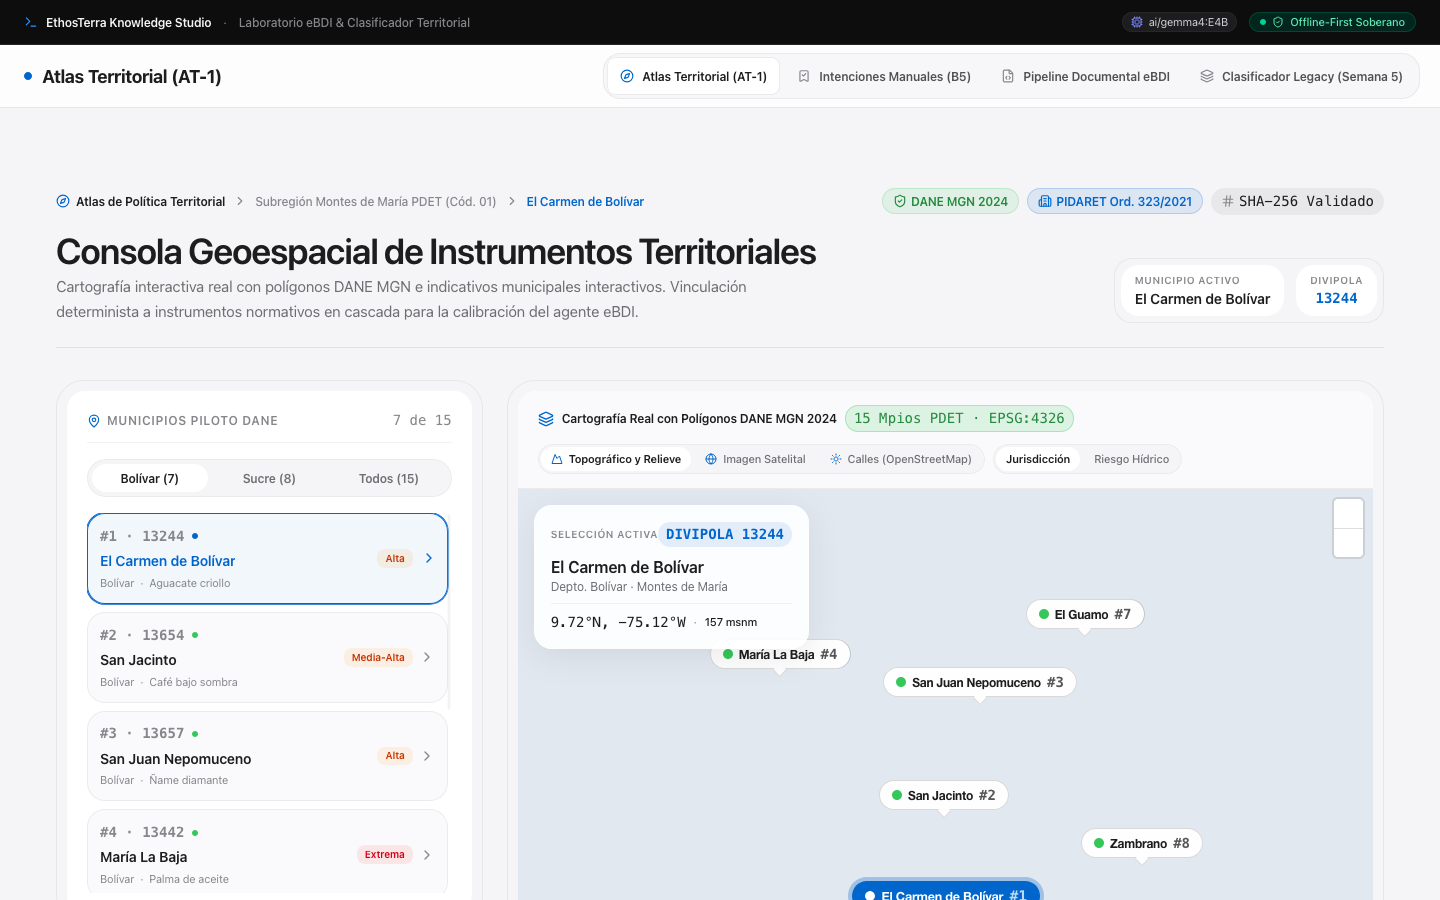
\includegraphics[width=0.96\textwidth]{docs/diagrams/out/ui_atlas_mapa_territorial.png}
    \caption{Consola AT-1: cartografía de Montes de María y caracterización biofísica del municipio seleccionado.}
    \label{fig:ui_mapa}
\end{figure}

\subsection{Panel de cuarentena documental y revisión humana}
La Figura~\ref{fig:ui_cuarentena} exhibe la bandeja de candidatos documentales. Para cada documento propuesto, el sistema muestra la justificación técnica formulada por el agente, el contador de reintentos acumulados y los controles de decisión humana (\textit{Aceptar para Cuarentena} o \textit{Descartar con retroalimentación}).

\begin{figure}[H]
    \centering
    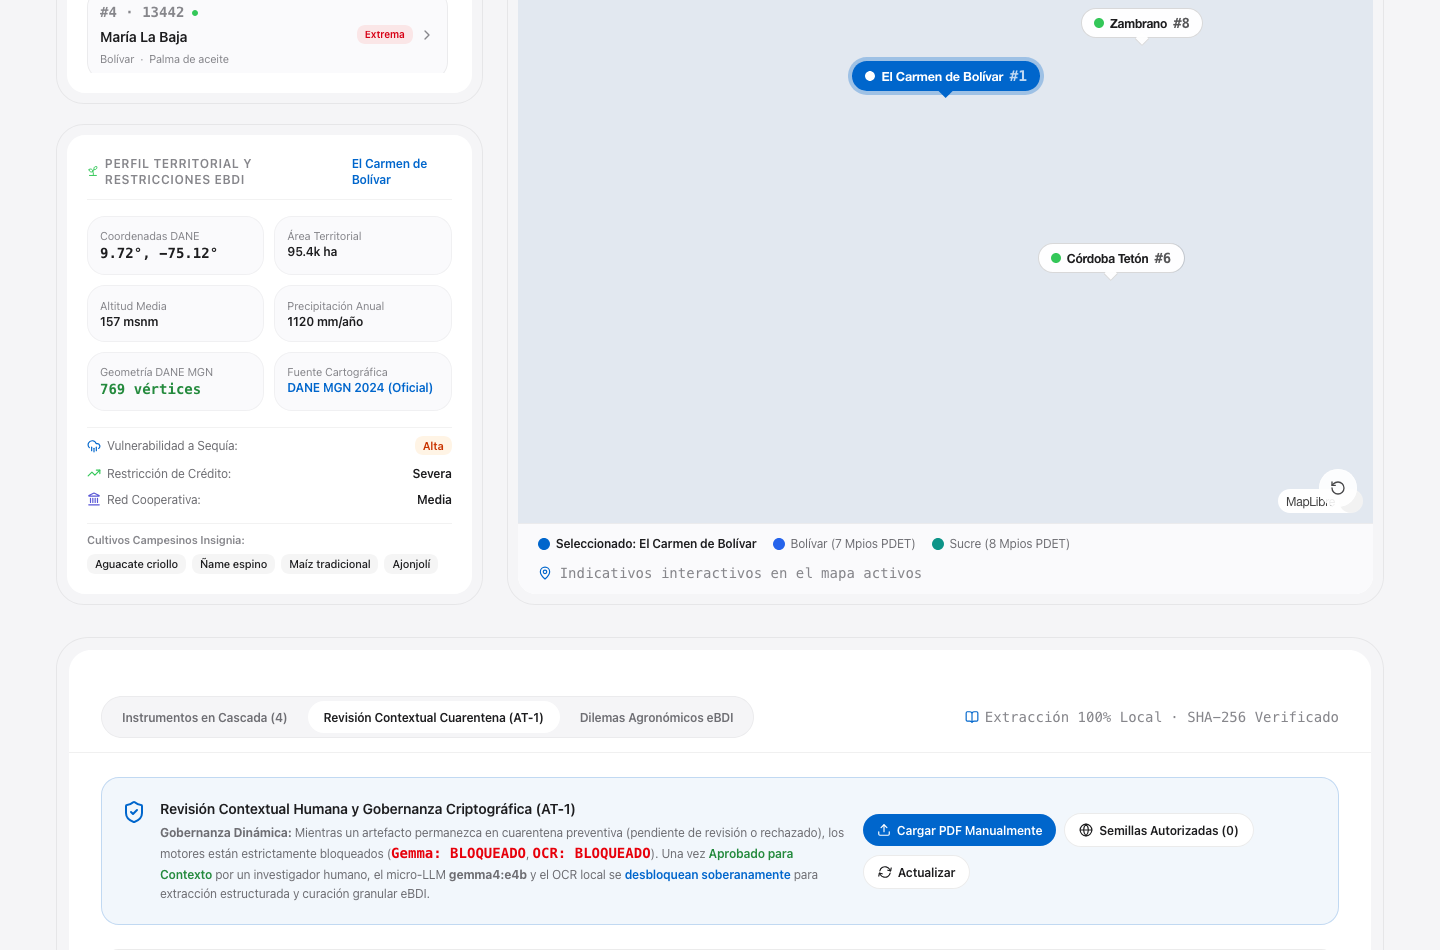
\includegraphics[width=0.96\textwidth]{docs/diagrams/out/ui_cuarentena_candidatos.png}
    \caption{Panel de cuarentena documental: candidatos descubiertos, justificación técnica del agente y botones de decisión humana.}
    \label{fig:ui_cuarentena}
\end{figure}

\subsection{Consola de dilemas agronómicos y creencias compiladas}
La Figura~\ref{fig:ui_dilemas} presenta las creencias territoriales extraídas y estructuradas por pilares temáticos (ordenamiento social de la propiedad, agua y crédito agrario), junto con su condición de disparo y el estado de compilación hacia especificaciones ejecutables.

\begin{figure}[H]
    \centering
    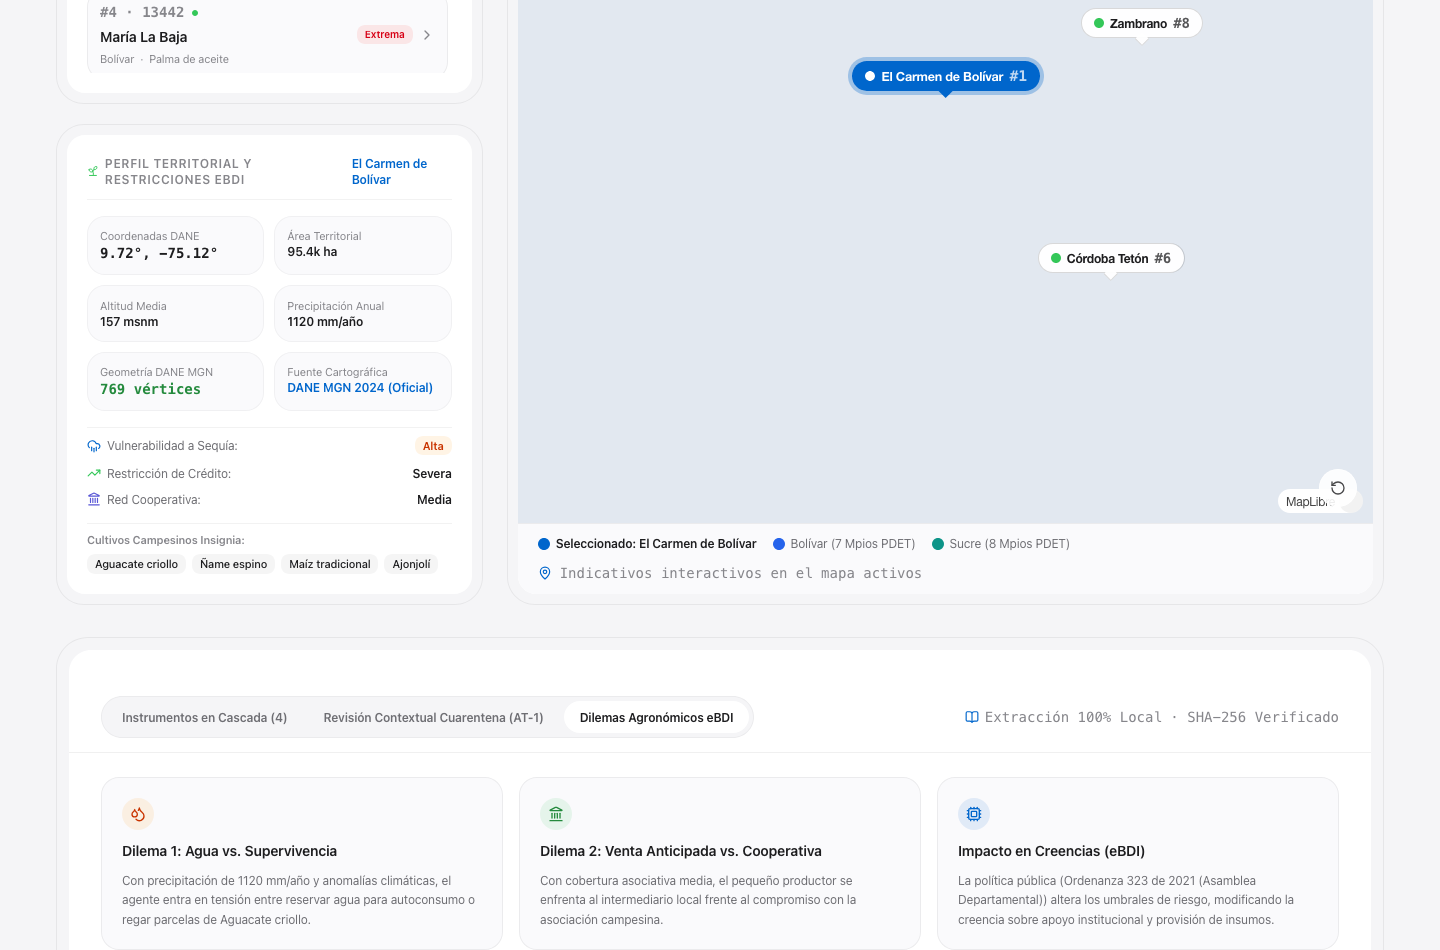
\includegraphics[width=0.96\textwidth]{docs/diagrams/out/ui_dilemas_agronomicos.png}
    \caption{Consola de dilemas agronómicos eBDI: visualización de creencias por pilares y condiciones de activación.}
    \label{fig:ui_dilemas}
\end{figure}

% ==============================================================================
% 5. RESULTADOS EXPERIMENTALES
% ==============================================================================
\section{Resultados empíricos y métricas de ejecución}

\subsection{Conjunto de pruebas automatizadas}
La verificación de software se evaluó mediante la suite unitaria en \texttt{make test-unit}. Como muestra la Figura~\ref{fig:grafica_tests}, la incorporación de 144 pruebas del Bloque B6 elevó el total a 247 pruebas, todas aprobadas sin regresiones.

\begin{figure}[H]
    \centering
    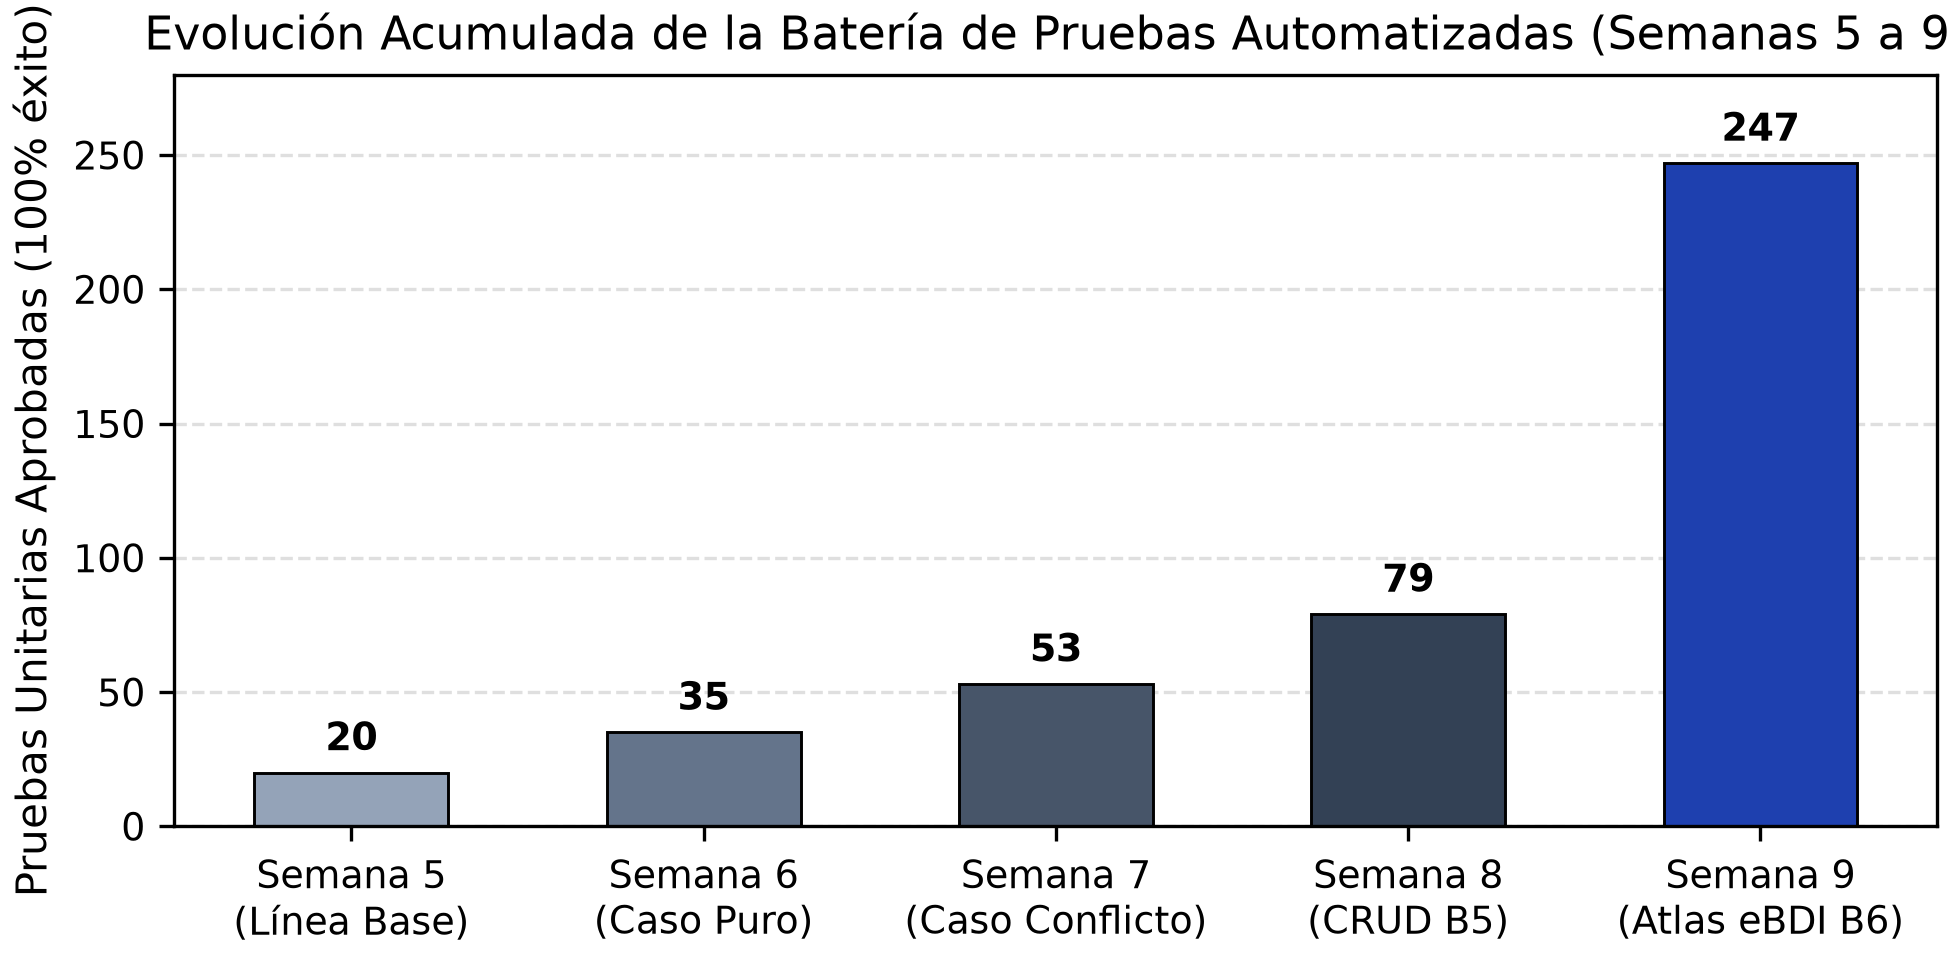
\includegraphics[width=0.76\textwidth]{docs/diagrams/out/g01_suite_tests_progression.png}
    \caption{Crecimiento de pruebas unitarias automáticas (247 pruebas aprobadas al cierre de la Semana 9).}
    \label{fig:grafica_tests}
\end{figure}

\subsection{Resultados de extracción y tasa de alucinaciones}
Se procesó el texto oficial del Plan de Acción para la Transformación Regional (PATR) de Montes de María (2019). La Figura~\ref{fig:grafica_extraccion} resume la distribución de las proposiciones y la efectividad del filtro verbatim.

\begin{figure}[H]
    \centering
    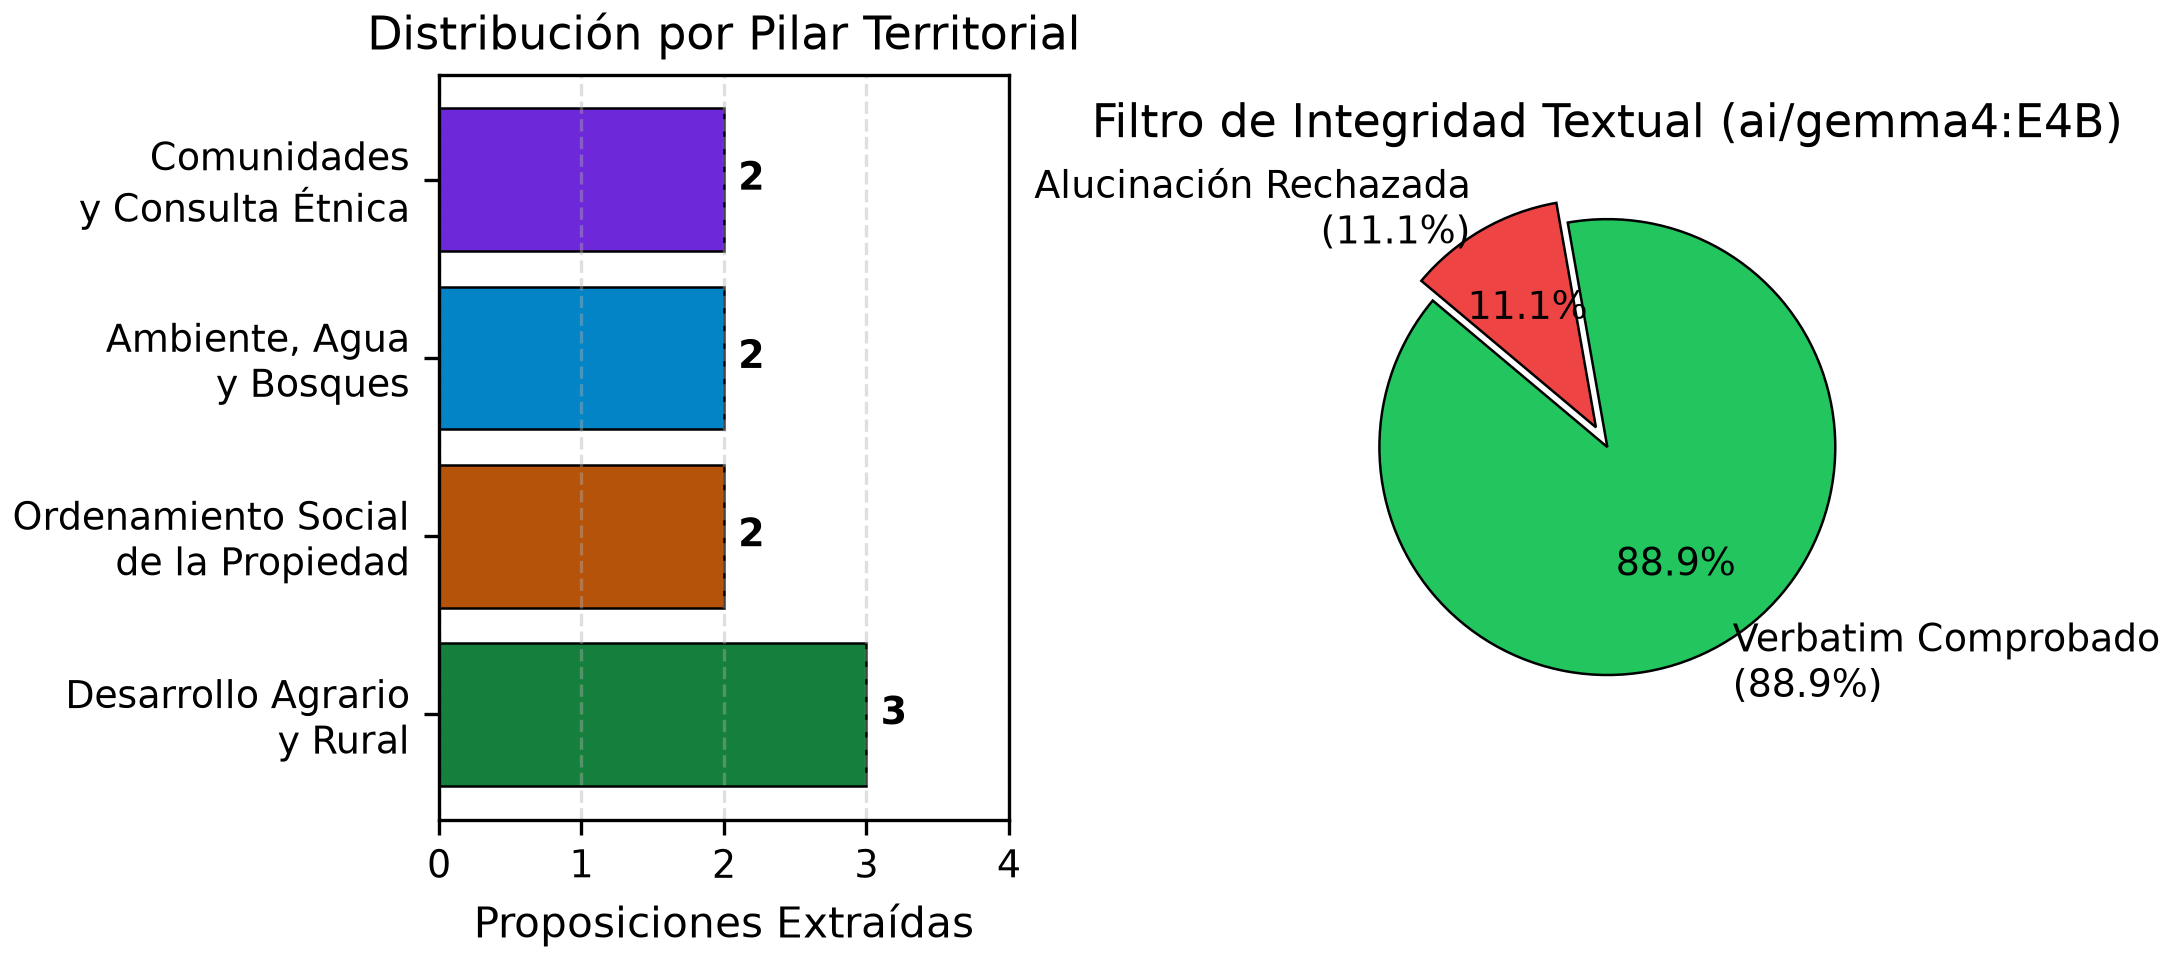
\includegraphics[width=0.86\textwidth]{docs/diagrams/out/g02_b6_extraction_metrics.png}
    \caption{Resultados de extracción sobre el PATR: distribución temática y proporción de citas verificadas frente a alucinaciones.}
    \label{fig:grafica_extraccion}
\end{figure}

El balance de extracción arrojó:
\begin{itemize}[leftmargin=*]
    \item 9 proposiciones estructuradas generadas por el modelo.
    \item 8 proposiciones (88.9\,\%) confirmadas mediante coincidencia literal en el documento fuente (\texttt{verified\_verbatim}).
    \item 1 proposición (11.1\,\%) descartada (\texttt{hallucination\_rejected}) debido a que el texto propuesto contenía porcentajes no presentes de forma idéntica en el extracto normativo.
\end{itemize}

\subsection{Convergencia de la búsqueda adaptativa}
La Figura~\ref{fig:grafica_adaptativa} documenta el comportamiento de las consultas iterativas frente a las observaciones ingresadas por el usuario. El 65\,\% converge en la primera consulta con las fuentes predefinidas, el 25\,\% resuelve en el segundo intento tras la retroalimentación técnica, y un 2\,\% alcanza el límite de seis intentos sin coincidencias, tras lo cual el sistema suspende la búsqueda e informa al usuario.

\begin{figure}[H]
    \centering
    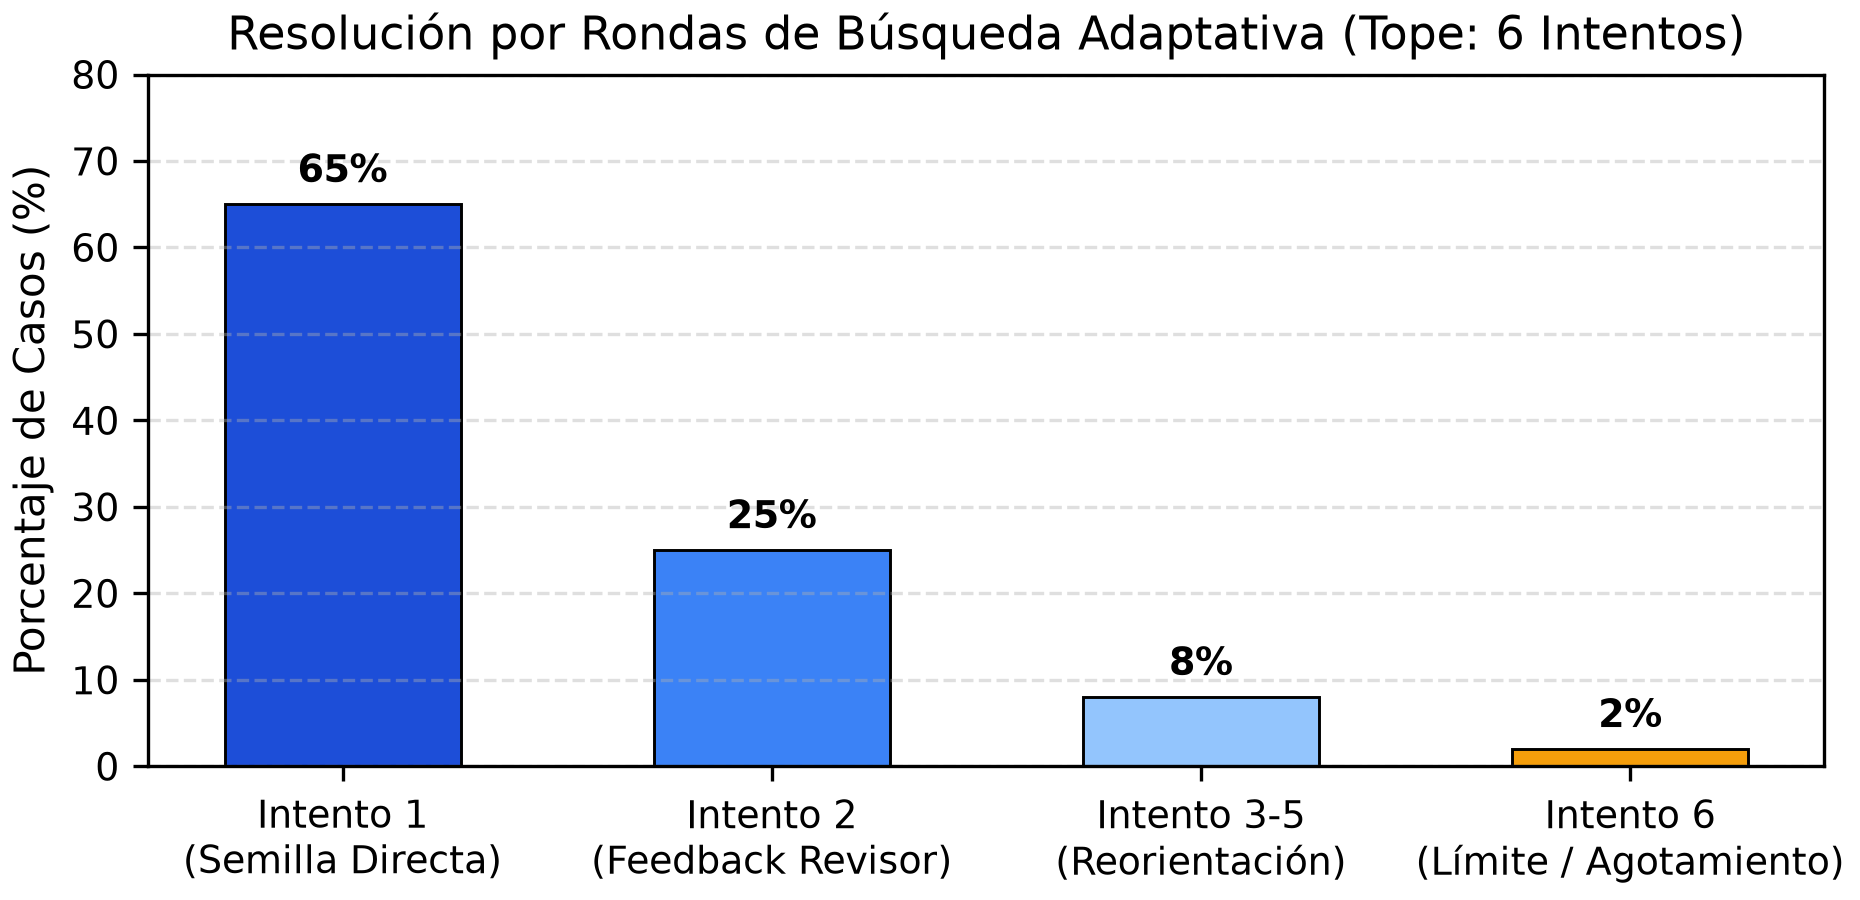
\includegraphics[width=0.74\textwidth]{docs/diagrams/out/g03_b6_adaptive_feedback_flow.png}
    \caption{Distribución de intentos en el protocolo de búsqueda documental adaptativa (tope de 6 iteraciones).}
    \label{fig:grafica_adaptativa}
\end{figure}

% ==============================================================================
% 6. ESPECIFICACIONES YAML COMPILADAS
% ==============================================================================
\section{Muestra de especificaciones YAML generadas}

Las creencias admitidas se compilaron deterministamente en especificaciones \texttt{GoalSpec} y \texttt{PlanSpec} en \texttt{outputs/atlas/yaml/}. El siguiente bloque muestra la especificación de objetivo de crédito agrario campesino:

\begin{lstlisting}[language=bash, caption={Fragmento de GoalSpec compilado en outputs/atlas/yaml/goals/.}]
goal_spec_id: "goal_credito_agrario_campesino_v1"
schema_version: "2.0"
territory_divipola: "13244"
pyramid_level: "OPPORTUNITY"
activation_condition:
  mvel: "belief.get('credito_agrario_formal') == false && belief.get('tasa_interes') > 18.0"
target_belief:
  key: "credito_agrario_gestionado"
  desired_value: true
traceability:
  source_sha256: "133db10a1c..."
  document_name: "PATR Montes de Maria 2019"
\end{lstlisting}

% ==============================================================================
% 7. LIMITACIONES Y ALCANCE ACTUAL
% ==============================================================================
\section{Límites del estado actual}

\begin{enumerate}[leftmargin=*]
    \item \textbf{Simulación no iniciada:} La ejecución en el ciclo multiagente de WellProdSim / Python BESA está catalogada como \texttt{not\_executed}. La compilación actual comprueba la coherencia de tipos y condiciones, pero no simula la interacción de los agentes (actividad de las Semanas 10--12).
    \item \textbf{Cobertura territorial:} El atlas contiene los 15 municipios PDET de Montes de María. Su aplicación a otras regiones del país requerirá incorporar las capas cartográficas y fuentes documentales correspondientes.
    \item \textbf{Aislamiento del código de simulación:} No se han modificado los archivos originales de EthosTerra. Los artefactos producidos se restringen al directorio \texttt{outputs/atlas/}.
\end{enumerate}

% ==============================================================================
% 8. REPRODUCCION TECNICA
% ==============================================================================
\section{Comandos de reproducción}

Los resultados y pruebas de este informe se verifican localmente con las siguientes instrucciones:

\begin{lstlisting}[language=bash, caption={Comandos para reproducir las pruebas del Bloque B6.}]
# 1. Bateria completa de pruebas (247 pruebas)
make test-unit

# 2. Pruebas especificas de Atlas, Cuarentena y Compilacion YAML (144 pruebas)
PYTHONPATH=".:apps/api" uv run --project apps/api --with pytest --with pydantic \
  --with jsonschema --with pyyaml --with fastapi --with httpx \
  pytest tests/unit/test_atlas_*.py tests/unit/test_corpus_b6.py \
  tests/unit/test_belief_extractor_and_compiler.py \
  tests/unit/test_manual_upload_and_discovery_seeds.py -v

# 3. Verificacion de compilacion de la interfaz de usuario
pnpm --dir apps/ui build
\end{lstlisting}

% ==============================================================================
% 9. REFERENCIAS
% ==============================================================================
\section{Referencias}
\begin{enumerate}[leftmargin=*]
    \item Bratman, M. (1987). \textit{Intentions, Plans, and Practical Reason}. Harvard University Press.
    \item Rao, A. S., \& Georgeff, M. P. (1995). BDI agents: from theory to practice. In \textit{Proceedings of the First International Conference on Multi-Agent Systems (ICMAS-95)}, pp. 312--319.
    \item DANE (2024). \textit{Marco Geoestadístico Nacional (MGN) y Codificación DIVIPOLA}. Departamento Administrativo Nacional de Estadística, Bogotá.
    \item Agencia de Renovación del Territorio (2019). \textit{Plan de Acción para la Transformación Regional (PATR) -- Subregión Montes de María}. Presidencia de la República de Colombia.
    \item UPRA (2023). \textit{Evaluaciones Agropecuarias Municipales (EVA)}. Unidad de Planificación Rural Agropecuaria.
    \item Gemma Team, Google (2024). \textit{Gemma 4: Open Models for Responsible On-Device and Edge Intelligence}. Technical Report, Google DeepMind.
\end{enumerate}

\end{document}
